
En este apéndice se especifican las instrucciones de instalación de la API en
un servidor en producción. Todos estos pasos están incluidos en el repositorio
de configuración de Vagrant.\cite{repo-vagrant}

\section{Requisitos previos}

Para poder desplegar correctamente el sistema en un servidor, este debe cumplir
con los siguientes requisitos mínimos.

\subsection{Hardware}

\begin{itemize}
\item 512 MiB de memoria RAM
\item 10 GiB de disco duro
\item Acceso a internet con un canal de subida de al menos 1 Mbit/s
\end{itemize}

\subsection{Software}

\begin{itemize}
\item Sistema operativo GNU/Linux. Este manual de instalación está optimizado
  para Ubuntu, pero puede utilizarse cualquier otra distribución.
\item Acceso mediante SSH.
\item Un usuario con permisos para poder ejecutar el comando \texttt{sudo}. En su
  defecto, podríamos loguearnos como \texttt{root}, pero no es seguro.
\end{itemize}

El resto de paquetería necesaria viene especificada en la instalación con cada
paso para instalarla y configurarla.


\section{Instalación inicial}

\subsection{Paquetería básica}

Necesitaremos actualizar la paquetería del sistema e instalar los paquetes
básicos, como Python o Git. Para ello hay que ejecutar los siguientes comandos.

\begin{minted}{bash}
$ sudo apt-get update
$ sudo apt-get install software-properties-common
$ sudo apt-get install python3-dev python3-pip python3-setuptools
$ sudo python3 -m easyinstall pip
$ sudo apt-get install python-psycopg2
$ sudo apt-get install git
$ sudo apt-get install supervisor
\end{minted}

\subsection{Descarga del código del repositorio}

Es necesario, obviamente, descargar el código del repositorio con el código
de la API.\cite{repo-serenity} Todos los comandos que se indican deben
ejecutarse desde el directorio \texttt{home} del usuario del servidor. Si se
decide optar por otra ruta, cada vez que haya que indicar el usuario en un
comando o archivo habrá que modificarla por la que hayáis elegido.

\begin{minted}{bash}
git clone https://github.com/nessa/serenity.git ~/serenity
\end{minted}


\subsection{Instalación del servidor web}

Esta guía está preparada para utilizar \textbf{nginx}, pero podría utilizarse
\textit{Apache}.

\begin{minted}{bash}
$ sudo apt-get install nginx
\end{minted}

El siguiente paso es crear el archivo \texttt{/etc/nginx/sites-available/serenity}
con el siguiente contenido, sustituyendo \texttt{<dominio>} por vuestro dominio y
\texttt{<usuario>} por el usuario con el que estéis logueados en el servidor:

\begin{minted}{bash}
server {
        listen 80;
        server_name <dominio>;

        error_log /var/log/nginx/error.log;
        access_log /var/log/nginx/access.log;


        location /static {
                alias /home/<usuario>/serenity/amuseapi/static;
        }

        location / {
                proxy_set_header X-Forwarded-Host $server_name;
                proxy_set_header X-Real-IP $remote_addr;
                add_header P3P 'CP="ALL DSP COR PSAa PSDa OUR NOR ONL UNI COM NAV"';
                proxy_pass http://127.0.0.1:8001/;
        }
}
\end{minted}

A continuación hay que enlazar dicho archivo como un sitio activado de nginx:

\begin{minted}{bash}
$ sudo ln -s /etc/nginx/sites-available/serenity
    /etc/nginx/sites-enabled/serenity
$ sudo service nginx restart
\end{minted}


\subsection{Instalación del servidor de bases de datos}

En nuestro caso, vamos a configurar PostgreSQL:

\begin{minted}{bash}
$ sudo apt-get install libpq-dev python-dev python-psycopg2
$ sudo apt-get install postgresql postgresql-contrib
$ sudo service postgresql start
\end{minted}

Cambiamos de usuario a \texttt{postgres} para configurar la contraseña de un
nuevo usuario de base de datos y crear la nueva base de datos (indicad el nombre
de usuario y contraseña que queráis):

\begin{minted}{bash}
$ sudo su postgres 
$ createuser <usuario>
$ createdb -O <usuario> <db>
$ psql db
$ ALTER USER "<usuario>" WITH PASSWORD '<new_password>';
\end{minted}


\subsection{Creación de archivos de log}

Es importante tener los archivos de log bien localizados, así que vamos a
crearlos y darles permisos.

\begin{minted}{bash}
$ sudo mkdir  /var/log/django
$ sudo touch /var/log/django/serenity.log
$ sudo chown -R usuario:usuario /var/log/django/
$ sudo chmod -R u+x /var/log/django/serenity.log
$ sudo chmod -R go+w /var/log/django/serenity.log
\end{minted}


\subsection{Instalación del entorno Gunicorn}

Generamos un nuevo entorno virtual:

\begin{minted}{bash}
$ sudo pip install --upgrade pip
$ sudo pip3 install virtualenv
$ virtualenv gunicorn-env
$ source gunicorn-env/bin/activate
$ pip3 install -r serenity/amuseapi/reqs/all.txt
\end{minted}

Creamos el archivo \texttt{gunicorn-env/exec} con el siguiente contenido:

\begin{minted}{bash}
#!/bin/bash
source /home/usuario/gunicorn-env/bin/activate
$@
\end{minted}

Y damos permisos al archivo:

\begin{minted}{bash}
$ chmod a+w  gunicorn-env/exec 
$ chmod u+x  gunicorn-env/exec
\end{minted}


\subsection{Despligue de ficheros estáticos}

Creamos nuestro archivo de configuración personalizado en
\\ \texttt{/etc/serenity-settings.ini}
con el siguiente contenido, indicando el nombre de la base de datos (en lugar de
\texttt{<db\_name>}), el del usuario de la base de datos (en lugar de
\texttt{<db\_user>}) y la contraseña (en lugar de \texttt{<db\_password>}).
También especificamos una clave secreta (en lugar de
\texttt{<secret\_key>}).\footnote{La clave puede generarse en la siguiente URL:
  \url{http://www.miniwebtool.com/django-secret-key-generator/}.}

\begin{minted}{bash}
[database]
DATABASE_NAME:<db_name>
DATABASE_USER:<db_user>
DATABASE_PASSWORD:<db_pass>

[secret]
SECRET_KEY:<secret_key>
\end{minted}

Cambiamos los permisos del archivo:

\begin{minted}{bash}
$ sudo chown usuario:usuario /etc/serenity-settings.ini
\end{minted}

Y utilizamos un comando de Django para generar todos los ficheros estáticos:

\begin{minted}{bash}
$ /home/nessa/gunicorn-env/exec python /home/nessa/serenity/amuseapi/manage.py
  collectstatic --noinput
\end{minted}

\subsection{Configuración de Supervisor}

Creamos el archivo \texttt{gunicorn\_start} con el siguiente contenido:

\begin{minted}{bash}
#!/bin/bash
NAME="serenity"
DJANGODIR=/home/<usuario>/serenity/amuseapi
USER=<usuario>
NUM_WORKERS=3


# Activate the virtual environment
source /home/<usuario>/gunicorn-env/bin/activate

#Export pythonpath
export PYTHONPATH=/home/<usuario>/serenity/amuseapi/static:$PYTHONPATH

# Start your Django Unicorn
# Programs meant to be run under supervisor should not daemonize
# themselves (do not use --daemon)
exec gunicorn -c /home/vagrant/gunicorn-config amuseapi.wsgi:application
     --pythonpath /home/<usuario>/serenity/amuseapi
     --log-level debug
     --access-logfile gunicorn_access.log
     --log-file gunicorn_logfile.log
     --error-logfile gunicorn_errors.log
\end{minted}


Y el archivo gunicorn-config con este:

\begin{minted}{bash}
command = '/opt/myenv/bin/gunicorn'
pythonpath = '/opt/myenv/myproject'
bind = '127.0.0.1:8001'
workers = 3
\end{minted}

Creamos también el archivo de configuración de supervisor:

\begin{minted}{bash}
[program:serenity]
command = /home/<usuario>/gunicorn_start
user = root
stdout_logfile = /home/<usuario>/gunicorn_supervisor.log
redirect_stderr = true
environment=LANG=en_US.UTF-8,LC_ALL=en_US.UTF-8
\end{minted}

Y cambiamos los permisos y reiniciamos los servicios:

\begin{minted}{bash}
$ sudo chmod a+x gunicorn_start
$ sudo service supervisor start
$ sudo supervisorctl reread
$ sudo service supervisor restart
\end{minted}

\subsection{Migración de la base de datos}

Por último, migramos la base de datos:

\begin{minted}{bash}
$ /home/nessa/gunicorn-env/exec python \
    /home/nessa/serenity/amuseapi/manage.py migrate
\end{minted}

Si accedes al dominio configurado, deberías ver la página principal de la API:

\begin{figure}[htbp]
  \centering
  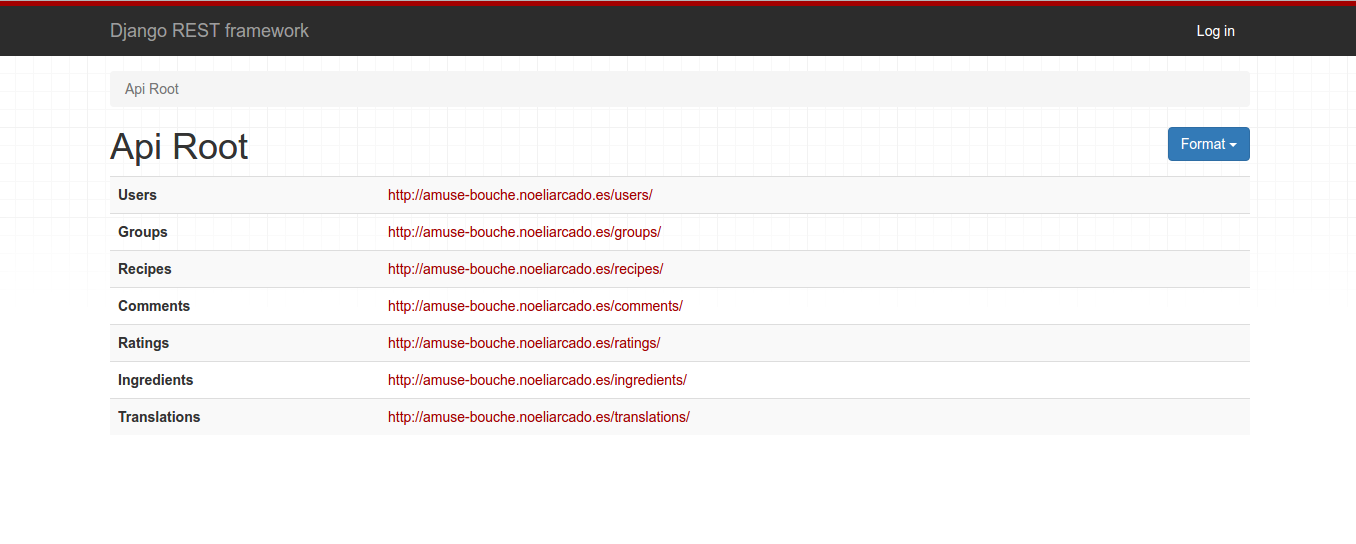
\includegraphics[width=\textwidth]{apen1/img/api}
  \caption{}
  \label{fig:api-web}
\end{figure}
